\subsection{Сборка}

Основным этапом стала сборка итогового устройства.

Электрическая схема была собрана из: шагового мотора, платы-драйвера шагового мотора, Arduino Nano, фототранзистора, ИК-светодиода, LCD экрана формата 2004 вместе с платой I2C, 2-х кнопок и провода USB (для питания). Схема соединений приведена ниже на рисунке (\ref{ris:scheme_electric})

\begin{figure}[H]
	\centering
	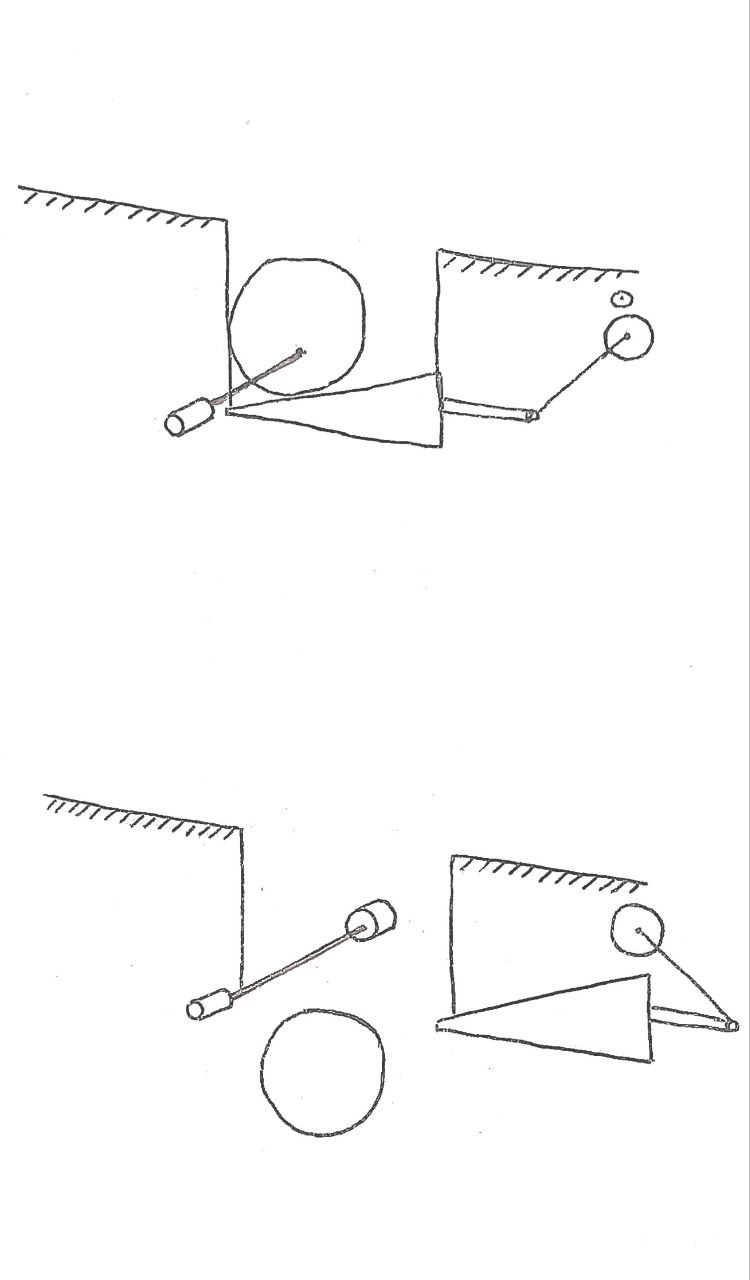
\includegraphics[width=12cm]{scheme_idea.jpg}
	\caption{Схема соединения проводов}
	\label{ris:scheme_electric}
\end{figure}





Основным этапом стала сборка электрической схемы устройства. 

Электрическую схему!

Паяли-запаяли-заклеили. 

Пружинку и проволку!

